\documentclass{article}



\usepackage{arxiv}

\usepackage[utf8]{inputenc} % allow utf-8 input
\usepackage[T1]{fontenc}    % use 8-bit T1 fonts
\usepackage{hyperref}       % hyperlinks
\usepackage{url}            % simple URL typesetting
\usepackage{booktabs}       % professional-quality tables
\usepackage{amsfonts}       % blackboard math symbols
%\usepackage{nicefrac}       % compact symbols for 1/2, etc.
\usepackage{microtype}      % microtypography
\usepackage{lipsum}		% Can be removed after putting your text content
\usepackage{graphicx}
\usepackage{natbib}
\usepackage{doi}
\usepackage{listings}



\title{Quantifying uncertainty in Pareto lake area estimates}

%\date{September 9, 1985}	% Here you can change the date presented in the paper title
%\date{} 					% Or removing it

\author{ \href{https://orcid.org/0000-0002-5924-2464}{
\includegraphics[scale=0.06]{orcid.pdf}\hspace{1mm}J.~Stachelek}\thanks{\href{https://jsta.rbind.io}{https://jsta.rbind.io}} \\
	Center for Limnology\\
	University of Wisconsin-Madison\\
	Madison, WI 53706 \\
	\texttt{stachelek@wisc.edu} \\
}

% Uncomment to remove the date
%\date{}

% Uncomment to override  the `A preprint' in the header
%\renewcommand{\headeright}{Technical Report}
%\renewcommand{\undertitle}{Technical Report}
\renewcommand{\shorttitle}{Pareto lake area uncertainty}

%%% Add PDF metadata to help others organize their library
%%% Once the PDF is generated, you can check the metadata with
%%% $ pdfinfo template.pdf
\hypersetup{
pdftitle={Quantifying uncertainty in Pareto lake area estimates},
pdfsubject={stat.AP},
pdfauthor={J.~Stachelek}
}

\begin{document}
\maketitle

\begin{abstract}
	Size is a critical factor determining the rate and occurrence of specific lake processes such as carbon sequestration and greenhouse gas emissions. Because we do not have a complete census of all lakes, upscaling estimates of such processes at broad spatial scales requires the use of lake size-abundance distributions rather than empirical measurements of area. Existing lake census efforts are incomplete such that as lakes become smaller they are more likely to by omitted either because they are too small to be resolved from remote sensing products or because of limited ground surveying effort (i.e. "censoring" of small lakes relative to large lakes).

The present study explores one potential shortcoming of prior approaches estimating global lake area using lake size-abundance distributions. Namely, these prior approaches rely on frequentist curve fitting techniques combined with an ad-hoc cutoff determination strategy (visual inspection to determine a likely censoring point). This yields an over-exact lake area estimate that is overwhelmingly reported with no uncertainty bounds. I address this shortcoming by fitting models in a Bayesian framework where each parameter contributes uncertainty to model estimates. I show that such although such models produce a more realistic estimate of lake area uncertainty they underestimate true total lake area. The degree of this underestimation is likely related to the proportion of the dataset subject to censoring. Ultimately, this may explain the fact that total lake area estimates have increased through time as the resolution of lake databases has improved.
\end{abstract}

\section{Introduction}
Size is a critical factor determining the contribution of lakes to global biogeochemical cycling and existing evidence suggests that lakes are key components of overall carbon burial, sequestration, and greenhouse gas emissions \citep{delsontroGreenhouseGasEmissions2018, kellerGlobalCarbonBudget2021}. The calculation of such fluxes requires two terms 1) an areal flux rate and 2) the distribution of total lake area. As with all estimates at broad spatial scales, uncertainty estimates are of great interest both because they allow for intercomparisons among similar lake studies and because they allow for comparisons between lakes and other ecosystems.

The techniques typically used to determine uncertainty in areal flux rates and the techniques typically used to determine uncertainty in total lake area distributions differ greatly. In the former case, uncertainties can typically be calculated in straightforward manner from literature compilations \citep{delsontroGreenhouseGasEmissions2018, kellerGlobalCarbonBudget2021}. In the latter case, uncertainty in total lake area distributions is challenged by the fact that no existing database is a complete census of all lakes \citep{messagerEstimatingVolumeAge2016} and the distribution of individual lake areas spans a range of approximately 7 orders of magnitude. The largest lakes are so big they could otherwise be classified as inland seas (> $10^4$ $km^2$) while the smallest are barely larger than a regulation sized soccer field (> $10^{-3}$ $km^2$).
A consequence of these challenges is that uncertainty varies within the distribution as a function of lake size. The area of the largest lakes is known exactly while the area of the smallest lakes is incomplete below a certain unknown threshold. This can occur either because lakes are too small to be resolved from remote sensing products or because of limited ground surveying effort. The omission or "censoring" of small lakes occurs because we know that small lakes exist but below a certain threshold we have limited knowledge of their exact areas \citep{hamiltonEstimationFractalDimension1992}.

Estimating total lake area from a sample of lakes requires a conceptual model of how lakes are formed (i.e. the data generating process). Typically, lake areas are treated as arising from a fractal generating process due to the fact that landform topography, which determines the placement of lakes, can itself be treated as a fractal generating process. Indeed, many other geomorphological phenomena that are dependent on landform topography such as coastline length are often well-described by fractal generating processes \citep{newman_power_2005}. A challenge in modelling such data generating processes for lake areas is large lakes likely follow a different data generating process than that of the smallest lakes. Whereas small lakes are constrained by landform topography, large lakes are essentially unconstrained by local landform topography and are instead constrained by the placement and arrangement of continents \citep{goodchildLakesFractalSurfaces1988}. As large lakes become even larger, they have a greater probability of intersecting a continent edge and becoming an estuary or embayment rather than a lake. Consquently, lake databases are said to be truncated on large lakes because we know that large lakes are essentially fixed in space and cannot occur in any given location \citep{hamiltonEstimationFractalDimension1992}.

From the preceding discussion it is clear that estimating total lake area requires a method of dealing both with the fact that lake databases are 1) truncated at large lakes and 2) censored at small lakes. Previous studies estimating global lake area have essentially not dealt with the first issue but instead modified their estimation process to limit its effect on the results (see methods section). They have dealt with the second issue by specifying an ad-hoc cutoff value below which empirically determined lake areas are discarded and subsequently back calculated. Hereafter, I refer to this strategy as the cutoff method. In the present study, I explore the effects of using the typical frequentist approach for estimating total lake area (i.e. the cutoff method) via a simulation study. In addition, I demonstrate an approach to produce uncertainty estimates of total lake area in a Bayesian framework. I evaluate the effects of the cutoff method on a simulated dataset because it is not sensitive to other potential confounding factors such as heterogeneity of survey effort or data precision.

\section{Methods}

Lake areas are typically treated as arising from a scale-invariant fractal generating process \citep{winslowDoesLakeSize2015, downingGlobalAbundanceSize2006, mcdonald_regional_2012, goodchildLakesFractalSurfaces1988, hamiltonEstimationFractalDimension1992}. Essentially, this means that the number of lakes in one size class is proportional to the number of lakes in the preceding size class irrespective of their magnitudes. The numerical form describing such a process is a power-law function. One of the statistical tools often used to model data that follow a power-law function is the Pareto distribution which has a probability density function (pdf) of:

\begin{equation}
    pdf(A) = \alpha x_{min}^{\alpha}A^{-(\alpha+1)} \\
  \label{eqn:pareto_pdf}
\end{equation}

where $A$ is lake area, $a$ controls the “shape” of the distribution and $x_{min}$ controls the “scale” of the distribution \citep{shaliziAdvancedDataAnalysis2017}. Lake area studies using the Pareto distribution do not typically use the pdf directly. Instead, they use the inverse (complementary) cumulative distribution function (ccdf) (i.e. quantile function):

\begin{equation}
    ccdf(A) = \frac{x_{min}}{(1-A)^{\frac{1}{\alpha}}}
  \label{eqn:pareto_ccdf}
\end{equation}

The reason for using the ccdf is two-fold. First, it stabilizes model estimates in the lower tail of the distribution \citep{newman_power_2005}. This can be seen from the simulated data in Figure \ref{fig:pareto_demo} where the Pareto pdf contains a lot of noise in the tail but the ccdf appears smoothed. The smoothing of the tail is also desirable because it functions as a way of dealing with the truncated nature of lake databases. The second reason for using the ccdf is that it provides a computational shortcut for estimating the Pareto shape parameter $a$ because it is numerically equivalent to the slope of the ccdf in log-log space \citep{downingGlobalAbundanceSize2006}.

\begin{figure}
	\centering
	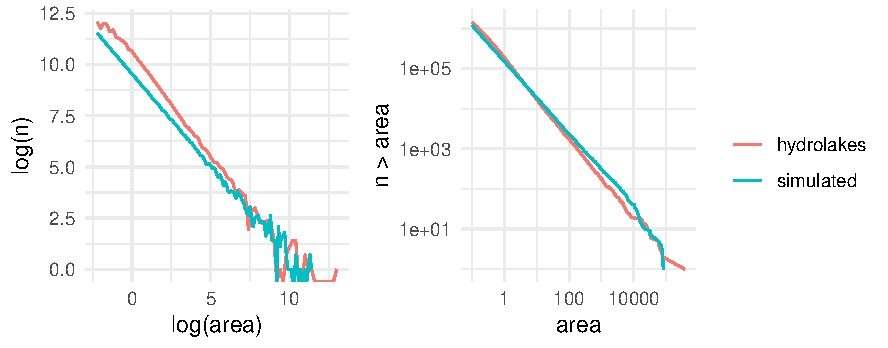
\includegraphics{figures/pareto_demo-1}
	\caption{Realization of a Pareto (A) probability density function and (B) complementary cumulative distribution function.}
	\label{fig:pareto_demo}
\end{figure}

For evaluation purposes, I generated a simulated dataset of 10,000 lake areas following the Pareto distribution using inverse transform sampling \citep{newman_power_2005}. Lakes in my simulated dataset have a minimum and maximum area of approximately 1 and 81000 $km^2$ respectively. This maximum was chosen to be approximately as large as Lake Superior but less than the Caspian Sea following \citet{lehnerDevelopmentValidationGlobal2004}. The "true" total area of these lakes is approximately 230000 $km^2$. I simulated a censored lake dataset by excluding lakes smaller than $e^{1}$. This excludes (censors) approximately 60\% of the total dataset. I approximated the "true" lake area total by constructing the empirical distribution function (edf) of the data which approximates the underlying Pareto cdf \citep{newman_power_2005}. Then I used this estimate of the cdf slope to generate cdf estimates for the censored lakes. I combined these cdf estimates with the edf values from the known lakes before calculating the sum of the inverted distribution (Figure \ref{fig:predict_area}).

I estimated the Pareto shape parameter $a$ in a frequentist framework by calculating the the slope of the edf in log-log space using linear regression in \texttt{R} \citep{team2013r}. I evaluated uncertainty in both $a$ and total lake area in a Bayesian framework using Stan \citep{standevelopmentteamStanModelingLanguage2017}. Instead of computing on the edf (as in the frequentist case), I computed directly on the pdf with the following Stan model:

\begin{minipage}[c]{0.95\textwidth}
\begin{lstlisting}
data {
  int<lower=0> N;
  real x[N];
}
parameters {
  real<lower=0> alpha;
  real<lower=0> xmin;
}
model {
  real lpa[N];

  xmin ~ gamma(.001, .001);
  alpha ~ gamma(.001, .001);

  for (i in 1:N) {
    lpa[i] = pareto_lpdf(x[i] | xmin, alpha);
  }

  target += sum(lpa);
}
\end{lstlisting}
\end{minipage}

I used uninformative gamma priors for both the $x_{min}$ and $a$ parameters following \citet{scollnikCompositeLognormalParetoModels2007}. I ran the model with four chains of 8,000 iterations and used the Stan defaults for burn-in and thinning which specify a burn-in of half the iterations and no thinning.

\section{Results}

Visual inspection of the frequentist method of computing on the edf appeared to produce a reasonable density estimate for small censored lakes (Figure \ref{fig:predict_area}). In addition, estimates of total lake area are somewhat close to the "true" value (Table \ref{tab:pred_table}). However, uncertainty around the frequentist estimates is unrealistically small (Figure \ref{fig:frequentist_uncertainty}).

\begin{figure}
	\centering
	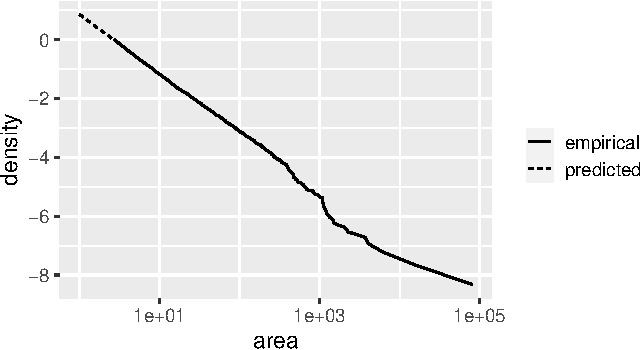
\includegraphics{figures/predict_area-1}
	\caption{Censored lake area edf (solid line) and cdf estimate (dashed line).}
	\label{fig:predict_area}
\end{figure}

\begin{figure}
	\centering
	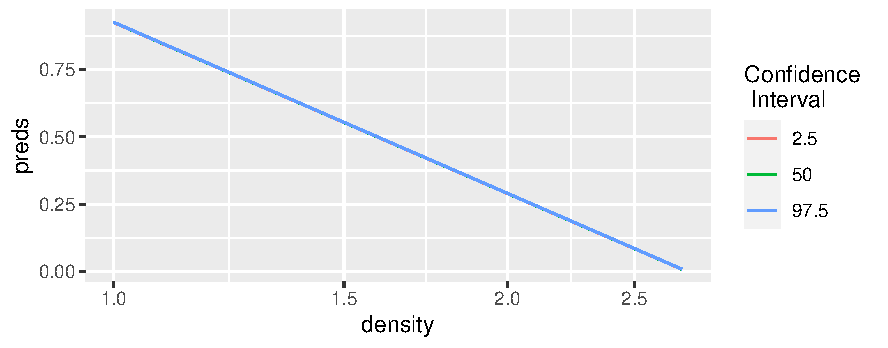
\includegraphics{figures/frequentist_uncertainty-1}
	\caption{Confidence interval of frequentist density predictions for censored data (the dashed portion in Figure 2. The confidence interval here has essentially no width.}
	\label{fig:frequentist_uncertainty}
\end{figure}

\begin{figure}
	\centering
	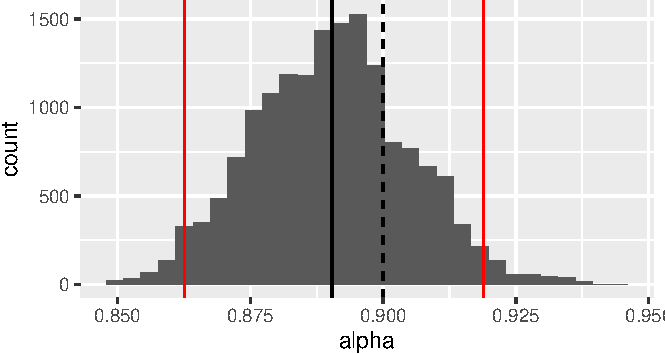
\includegraphics{figures/bayesian_model-1}
	\caption{Median (black line) and central 95 percent interval estimates of alpha (red lines). Here the 'true' alpha is 0.9.}
	\label{fig:bayesian_model}
\end{figure}

\begin{figure}
	\centering
	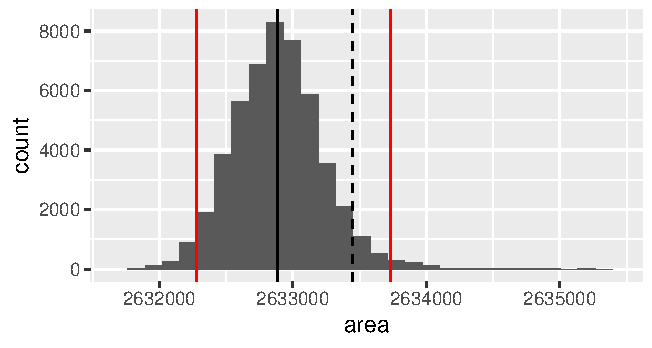
\includegraphics{figures/bayesian_area-1}
	\caption{Median (black line) and central 95 percent interval estimates of total lake area (red lines). Here the true total lake area is marked with a dashed vertical line.}
	\label{fig:bayesian_area}
\end{figure}

Instead of the essentially fixed $a$ and total lake area estimates produced by the frequentist approach, I found a substantial variability in both $a$ (95\% CI: 0.86, 0.92) and total area using a Bayesian approach (Fig \ref{fig:bayesian_model}, \ref{fig:bayesian_area}). In particular, the Bayesian 95\% credible intervals for both $a$ and total lake area encapsulate the true values (Fig \ref{fig:bayesian_model}, \ref{fig:bayesian_area}). Despite better uncertainty estimates using a Bayesian approach, both the frequentist and Bayesian approaches underestimated the true value of $a$ and total lake area.

\begin{table}
	\caption{'True' total lake area from the uncensored edf and estimated lake area from a combination of the censored edf and the estimated cdf.}
	\centering
	\begin{tabular}{cc}
	\toprule
		True Area ($km^2$) & Estimated Area ($km^2$) \\
	\midrule
		2.271e+05 & 2.263e+05 \\
	\bottomrule
	\end{tabular}
	\label{tab:pred_table}
\end{table}

\section{Discussion}

I have shown that the typical frequentist cutoff method produces reasonable estimates of the density of small censored lakes but that it does not capture uncertainty in total lake area (Table \ref{tab:pred_table}, Figure \ref{fig:frequentist_uncertainty}). Furthermore, I have shown that models fit using a Bayesian approach indicate substantial uncertainty in both total lake area and the underlying Pareto shape parameter $a$ used to derive these estimates (Figure \ref{fig:bayesian_model}, \ref{fig:bayesian_area}).

Although the 95\% credible interval of the Bayesian total lake area estimates encapsulate the true total lake area, the median value underestimates the true total lake area (Figure \ref{fig:bayesian_area}). It is likely that such underestimation, would increase with a greater proportion of censoring. This may explain the steady increase in estimates of global lake area through time from approximately 3 to 5 million $km^{2}$ as lake area databases have improved their accuracy \citep{lehnerDevelopmentValidationGlobal2004, downingGlobalAbundanceSize2006, verpoorterGlobalInventoryLakes2014}. Future work on estimating global lake area should consider implementing a sensitivity analysis looking at the response of total area estimates to variation in the degree of censoring.

A caveat of the present study is that it is difficult to confirm whether or not any particular dataset follows a fractal generating or Pareto process without strong prior knowledge. Indeed data following many heavy-tailed distributions such as the lognormal or negative exponential can appear to be equivalent to power-law distributions such as the Pareto \citep{clausetPowerlawDistributionsEmpirical2009}. The results of the present study confirm that an apparent change in the shape of the lower tail of a lake area distribution does not necessarily indicate a change in the data generating process. Note that the simulation dataset analyzed herein \emph{is} a truly fractal generated dataset with a homogeneous data generating process yet a cursory look would seem to indicate a change of data-generating process in the lower tail (Figure \ref{fig:predict_area}).

In addition to a sensitivity analysis of censoring, future work might consider more complex models that treat lake areas as a mixture of a Pareto distribution for small lakes and either a negative exponential or lognormal distribution for large lakes. Such an approach has been demonstrated by \citet{bonabeau_scaling_1999-1} and \citet{scollnikCompositeLognormalParetoModels2007}. Both studies show that the point at which the distribution mixtures converge can provide valuable inference. In the case of lakes, such a convergence point may indicate a change in the data generating process such as the point at which lake areas are controlled by continent placement rather than fractal landscape morphology \citep{goodchildLakesFractalSurfaces1988, hamiltonEstimationFractalDimension1992}.

\bibliographystyle{jsta}
\bibliography{pareto-lakes}

\end{document}
